\chapter{探测器蒙特卡洛模拟}
\label{chapter:background}

为了寻找NLDBD这个极其稀有的事件,一个极低本底的探测环境是PandaXIII实验需要着重解决的问题。所以为了能够在探测器实际建造之前细致的研究探测器结构和材料对本底水平的研究,我们使用Geant4\supercite{Agostinelli:2002hh}作为主要的蒙特卡洛模拟框架,构建了模拟器的模型。通过这个模型我们可以细致的研究探测器各个组件以及环境对实验本底的贡献,并根据这些数据来调节探测器的各种各样参数以达成实验的设计目标。具体的模拟细节如下列小节所述。

\section{目标元素及模拟工具}

因为探测器的铜壁相对较厚,而且铜壁的材料可以制作的较为纯净,在考虑到铜壁的屏蔽效应后,来自铜壁外的$\alpha$射线和$\beta$射线基本不可能到达探测器内部的灵敏区域,所以需要主要考虑到的本底辐射为探测器铜壁内部原件的各种辐射以及环境和材料中的$\gamma$射线。因为$^{136}$Xe的NLDBD事件释放出来的总能量$Q_{\beta\beta}=2458$keV,探测器设计的相对能量分辨率是3\%FWHW(半高全宽),因而我们定义能量窗口($Q_{\beta\beta}-2\sigma$, $Q_{\beta\beta}+2\sigma$)为能量敏感区域(Region Of Interest, ROI),其中$\sigma$为探测器在$Q_{\beta\beta}$处的绝对能量分辨率。计算可得ROI范围为2395keV到2520keV,所以衰变能量落在这个能量范围附近的元素便是我们感兴趣的元素。

根据各种放射性元素的衰变能量和在自然界中的丰度,再结合既往有关$^{136}$Xe的
NLDBD实验研究结果可以得到,我们关心的主要本底来自于$^{214}$Bi的gamma衰变,其能量为2447.8keV,以及来自于$^{208}$Tl的gamma衰变,其能量为2615.keV。这两种元素分别属于$^{238}$U和$^{232}Th$的衰变链中,而这两种放射性元素在自然界中大量的存在,绝大多数的材料都或多或少的含有它们。除了这两种元素,$^{60}$Co可能会释放出1.33MeV和
1.17MeV的$\gamma$射线,虽然两者和能量约为2.5MeV,但是这两个射线相对独立,同时落在探测器敏感区域内的概率不大,在加上读出窗口的限制$^{60}$Co对实验的影响会变得更小,因而在后续的模拟中它并没有被着重研究。表\ref{tab:activities}给出了构建探测器的原料中Th,U的放射性活度。
\renewcommand\arraystretch{1.4}
\begin{table*}[tbh]
    \centering
    \begin{tabular*}{0.75\textwidth}{@{\extracolsep{\fill}}cccc}
        \hline
        \hline
        \multirow{2}{*}{\textbf{材料}} & \multicolumn{3}{c}{\textbf{放射性活度 ($\mu$Bq/kg)}}
      \\
                                   & $^{232}$Th & $^{238}$U  & $^{60}$Co \\ \hline
      铜                       & 0.2        &   0.75     &     100     \\
      PTFE                         & 0.1        &   4.94      &    -      \\
      不锈钢              & 0.32$\times$10$^3$          &    0.5$\times$10$^3$      &     2.6$\times$10$^3$     \\
      超纯水                          & 0.04          &     0.12      &     -     \\
      混泥土                     & 9.9$\times$10$^6$          &    4.4$\times$10$^6$   &    -    \\
        \hline
        \hline
    \end{tabular*}
    \caption{不同材料的放射性活度表。铜和PTFE的活动数据来自于文献\cite{Abgrall:2016cct},不锈钢的数据来自于文献\cite{LZ_CDR},超纯水的数据来自于PandaXIII的中期报告\cite{cdr},混泥土的数据来自于文献\cite{Zeng2014}。}
    \label{tab:activities}
  \end{table*}
  

PandaXIII模拟工作中我们使用了Geant4软件作为蒙特卡洛模拟框架。Geant4是由
CERN开发的基于C++的蒙特卡罗应用包,它主要用于模拟粒子在物质中发生的各种物理过程。它内置了做粒子追踪所需要的完整方法包括径迹追踪,探测器几何构建,物理模型和数据等等,其中物理过程中包含了极大能量尺度下各种粒子之间的相互作用,材料和元素的数据。该软件被广泛的应用在了核物理,高能物理,医学研究等等领域。

PandaXIII实验在Geant4软件框架的基础上二次开发了两个模拟框架以满足复杂的模拟需求,分别被称作BambooMC和RestG4。BambooMC是由上海交通大学基于
PandaXII暗物质实验的模拟需求开发改进而成,后者是REST软件\supercite{tomas2013development}的一个模块。我们使用这两种框架独立进行了背景模拟工作,并对两者的结果做了交叉检查以确保结果的正确性。本文中的模拟工作都是由BambooMC模拟框架完成的。

\section{探测器结构及本底来源}
\begin{figure}[tbh]
    \centering
    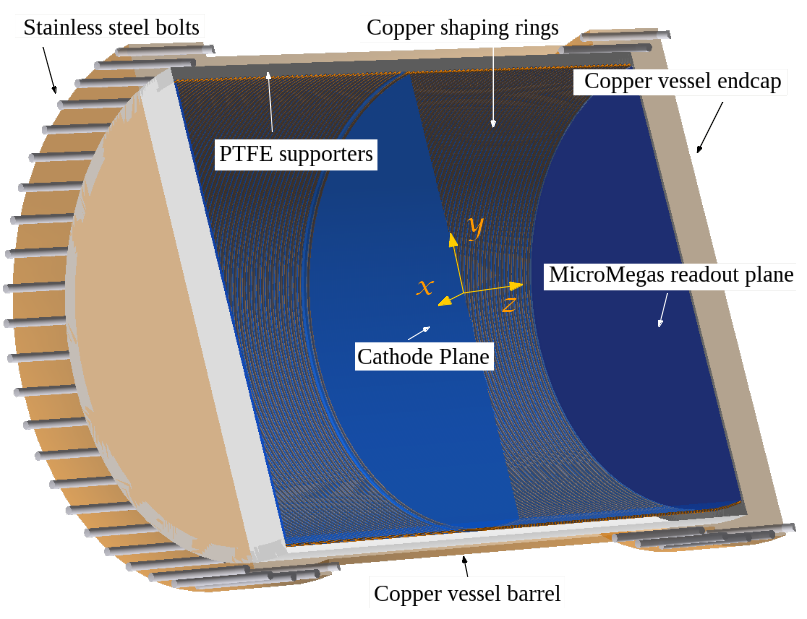
\includegraphics[width=0.4\columnwidth]{pic/fig3.png}
    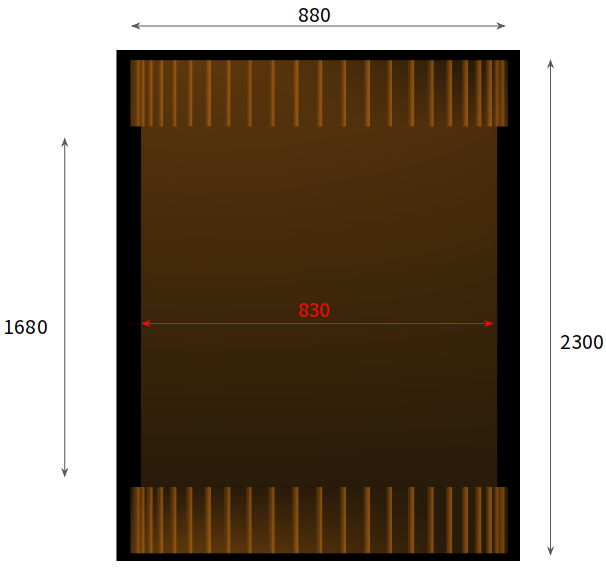
\includegraphics[width=0.4\columnwidth]{pic/fig5.png}
    \caption{左图:Geant4中PandaXIII背景模拟时间漂移室示意图\supercite{cnn},探测器被演奏平面切开。右图:铜罐结构的正视图以及外围尺寸。}
    \label{fig:detector_bamboomc}
\end{figure}

使用BambooMC构建出来的探测器结构如图\ref{fig:detector_bamboomc}所示。铜罐是由一个有法兰的圆柱体和两端的铜盖组成,每侧的铜盖和铜罐之间使用48个不锈钢螺钉铆和,铜罐壁厚度为3厘米,两端铜盖厚度为15厘米。在铜罐内部就是时间漂移室的主体结构,是由5cm厚度PTFE材料的作为支撑,延Z方向镶嵌99个管状圆形铜环组成的场笼,用于形成均匀的延Z方向的漂移电场。两个Micromegas读出平面放置在探测器的两端,同时中心的圆形铜极板将探测器分为上下两个漂移室。探测器主要原件的尺寸可以参照表\ref{tab:parameters_geometry}。
\begin{table*}[thb]
    \begin{center}
        \begin{tabular*}{0.75\textwidth}{@{\extracolsep{\fill}}ccccc}
        \hline
        \hline
        \textbf{组件} & \textbf{参数} & \textbf{值} & \textbf{材料} & \textbf{质量} \\ \hline
        \multirow{3}{*}{铜罐} & 内径 & 80\,cm & \multirow{3}{*}{铜} & \multirow{3}{*}{3438 kg} \\
                    & 高度 & 200\,cm &  &    \\   
                    & 壁厚 & 3\,cm &  &    \\\hline
        \multirow{2}{*}{铜盖} & 直径 & 88\,cm & \multirow{2}{*}{铜} & \multirow{2}{*}{3320 kg} \\
                    & 厚度 & 15\,cm &  &    \\\hline
        \multirow{2}{*}{螺钉} & 直径 & 1.4\,cm & \multirow{2}{*}{不锈钢} & \multirow{2}{*}{230.1 kg} \\
                    & 高度 & 40\,cm &  &    \\\hline
        \multirow{4}{*}{场笼} & 内径 & 75\,cm & \multirow{3}{*}{PTFE} & \multirow{3}{*}{1042 kg} \\
                    & 高度 & 200\,cm &  & \\ 
                    & 厚度 & 5\,cm &  & \\ 
                    & 铜环个数 & 99 &    \multirow{1}{*}{铜}  & 118.2 kg \\\hline
        中心极板 & 厚度   &   50\,$\mu$m     &   \multirow{1}{*}{铜}  &    0.79 kg   \\   
        \hline
        \hline
        \end{tabular*}
        \caption{探测器组成部件的几何参数,材料以及质量表。\supercite{cdr}}
        \label{tab:parameters_geometry}
    \end{center}
\end{table*}
  
探测器铜罐内填充了200kg的氙气与TMA混合气体,总体气压为10bar,被放置在中国锦屏地下实验室中的水池中。下列详细描述了探测器各个部分对本地的贡献:

\begin{description}
    \item[铜罐] 在模拟中我们将罐体和铜盖一起组成的压力铜罐容器作为了一个整体。虽然电解铜相对洁净(radiopure),但是它作为接近探测气体中最重的组件所产生的背景贡献不可忽略。模拟中使用的铜材料元素活度来自于表\ref{tab:activities}。
    \item[电子学] 因为大多数的电子学器件不可能做的相对洁净,电子学部分产生的本底辐射需要着重考虑,所以在实验的探测器设计中电子学部分被放置在15厘米厚的铜盖外侧以降低其对探测器的影响。在模拟中我们认为电子学$^{238}$U和$^{232}$Th的活度分别为0.26Bq和0.07Bq。此数据是来自于PandaXII暗物质实验的测量结果。
    \item[场笼]场笼是由5厘米厚的PTFE支撑以及等距嵌入的圆环做成的。整个场笼是探测器中质量使用更为仅次与铜罐的组件,其材料的放射性洁净也需要着重考虑,模拟中使用的数据参照表\ref{tab:activities}
    \item[不锈钢螺钉]在组合铜罐时我们使用了96个不锈钢螺丝钉。从表\ref{tab:activities}中可以看不锈钢的放射性洁净程度远远低于其他低本底材料,其活度比铜高了3个量级,因次虽然螺钉的整体质量相对较小,其对本底依然可能造成很大的影响。在模拟中不锈钢螺钉被简化为圆柱体以加速模拟的进行。
    \item[水池中的水]超纯水的放射性相对较低,同时因为水的自屏蔽现象,在模拟中我们只考虑了探测器周围5米范围内的衰变事件。
    \item[实验室水泥墙壁]从表\ref{tab:activities}可以看出水泥自身的放射性比铜高了6个量级,虽然探测器使用了水池来屏蔽,但我们依然需要通过模拟给出水池的最小尺寸以确保水泥及周边环境不会对实验造成过大影响。因为探测器和实验室墙壁之间有着$13\times11\times11$的水池作屏蔽,如果直接模拟水泥墙壁中$^{238}$U和$^{232}$Th的衰变,那么因为模拟效率和模拟数量的限制,基本上不可能有射线能够通过水池达到探测器,所以我们使用了下列的方式来估计实验室水泥墙壁的本底贡献:
    \begin{itemize}
        \item 第一步,我们模拟了在一块巨大的水泥块表面,由水泥内部$^{238}$U和$^{232}$Th产生的$\gamma$射线流的能谱。
        \item 第二步,我们将整个水池分为若干层,逐层的模拟。即根据上一步模拟得到的$\gamma$射线流的能谱,在第一层水的外表面均匀放置$\gamma$粒子,模拟得到穿过这一层水达到内表面的$\gamma$粒子的能谱,方向分布以及数目。随后在第二层的外表面根据第一层得到的粒子能谱和方向分布放置$\gamma$粒子,重复上述模拟过程。假设在第$i$层我们模拟了$N_i$个事件,只有$n_i$个穿过了水池被我们所记录,很容易得到$n_i<<N_i$。那么我们就可以定义$\alpha_i=N_{i+1}/n_i$为放大系数。即在第最后一层我们得到的模拟结果等价于我们不分层直接模拟$N_{eq}$个粒子,其中$$N_{eq}=N_0\Pi_{i=1}{t}a_i$$。其中$N_0$为起始模拟的粒子数目,t为总层数。
        \item 第三步,我们利用上一步中得到的最内层(约$2.5\times2.5\times2.5m^3$)的$\gamma$流能谱和方向分部信息,模拟并统计最终到达探测器内部气体的事件数目和能量分布,并由此计算总体对探测器本底的贡献。
    \end{itemize}
    在上述一层一层迭代的模拟过程中,因为我们关注的能量范围是2457.83keV,因而小于2.2MeV的能谱信息都会被直接忽略,这样可以大大加快计算的速度。
    \item[读出平面]PandaXIII实验中使用了Microbulk MicroMegas读出技术。而这种读出板自身是由低本底的铜以及Kapton塑料制造的。根据相关的实验测量数据,这种读出平面的
    $^{238}$U和$^{232}$Th的放射性约为$45nBq/cm^2$和$14nBq/cm^2$。
    \item[极板]探测器的极板是有铜制作的,而且它质量相对教轻,因次由它自身产生的放射性很低。但是气氙中所含有的部分$^{222}$Rn杂质有可能在电场的作用下富集到极板上,其衰变产物$^{214}$Bi会带来一定的背景信号。在模拟中我们假设Rn的含量为$1mBq/m^3$,即会造成基板上产生约$2nBq/cm^2$的$^{214}$Bi衰变。
\end{description}

我们使用BambooMC模拟框架模拟了上述各种组件对背景的贡献,蒙特卡洛模拟过程中,除了实验室水泥墙外其他组件是将待模拟的元素均匀的放置在结构中或表面上来作为初始粒子(primary particle),即进行了全链模拟(full-chain decay)。BambooMC模拟使用的物理过程是一个十分简答的考虑了衰变,电磁作用等物理过程,其启用了的模块如下:
\begin{itemize}
    \item G4EmLivermorePhysics
    \item G4EmExtraPhysics
    \item G4DecayPhysics
    \item G4RadioactiveDecayPhysics
    \item G4HadronElasticPhysicsHP
    \item HadronPhysicsShielding
    \item G4HadronPhysicsShielding
    \item G4StoppingPhysics
    \item G4IonQMDPhysics     
\end{itemize}

\begin{table*}[htb]
    \centering
    \begin{tabular*}{0.95\textwidth}{@{\extracolsep{\fill}}ccccc}
      \hline
      \hline
      \textbf{组件}&\textbf{元素}&\textbf{放射性活度}&\textbf{本底强度(计数/年)}&\textbf{ BI($10^{-5}c\/(keV\cdot kg\cdot y$))}\\
      \hline
      \multirow{2}{4em}{实验室水泥墙壁} & $^{238}$U  &  9.9 Bq/kg & $<0.40\pm0.03$  & -  \\
                                        & $^{232}$Th &  4.4 Bq/kg &  $<0.22\pm0.02$  & - \\ \hline
  
      \multirow{2}{4em}{水池} & $^{238}$U  & 0.12 $\mu$Bq/kg & 0.20 $\pm$ 0.1 &  0.74  \\
                                             & $^{232}$Th & 0.04 $\mu$Bq/kg & 0.24  $\pm$ 0.06 & 0.96 \\ \hline
      \multirow{3}{4em}{铜罐罐体}              & $^{238}$U  &  0.75 $\mu$Bq/kg & 1.73  $\pm$ 0.12 &  6.9  \\
                                             & $^{232}$Th & 0.2  $\mu$Bq/kg & 4.63  $\pm$ 0.18 & 18.5 \\
                                             & $^{60}$Co  & 10 $\mu$Bq/kg & 9.8  $\pm$ 1.0 &  39.0  \\ \hline
  
      \multirow{3}{4em}{铜罐盖子}            & $^{238}$U  & 0.75 $\mu$Bq/kg  & 0.83  $\pm$ 0.11 &  3.3 \\
                                             & $^{232}$Th & 0.2 $\mu$Bq/kg & 2.4  $\pm$ 0.1 &  9.8 \\
                                             & $^{60}$Co  & 10 $\mu$Bq/kg & 4.4  $\pm$ 1.0 &  17.8  \\ \hline
  
      \multirow{2}{4em}{不锈钢螺钉}              & $^{238}$U   &  0.5 mBq/kg & 7.5 $\pm$ 1.5 & 30.1  \\
                                            & $^{232}$Th  & 0.32 mBq/kg & 39.8 $\pm$ 2.7 & 159  \\ \hline
      \multirow{2}{4em}{场笼支撑体}    & $^{238}$U   & 4.94 $\mu$Bq/kg  & 15.0  $\pm$ 0.5  & 59.9 \\
                                            & $^{232}$Th  & 0.1 $\mu$Bq/kg & 2.69 $\pm$ 0.03 & 10.7  \\
      \multirow{2}{4em}{铜环}          & $^{238}$U  & 0.75 $\mu$Bq/kg  &  0.67 $\pm$ 0.01  & 2.7  \\
                                            & $^{232}$Th  & 0.2 $\mu$Bq/kg & 0.95 $\pm$ 0.01 &  3.8  \\ \hline
      \multirow{2}{4em}{电子学}        & $^{238}$U  & 0.26 Bq & 1.0 $\pm$ 0.3  & 4.2  \\
                                            & $^{232}$Th  & 0.07 Bq & 2.8 $\pm$ 0.2  & 11.3 \\ \hline
      \multirow{2}{4em}{Micromegas}         & $^{238}$U  & 45 nBq/cm$^2$ & 60.5 $\pm$ 1.7 &  241.6  \\
                                            & $^{232}$Th  & 14 nBq/cm$^2$ & 23.5 $\pm$ 0.6 &  93.9   \\ \hline
      \multirow{1}{4em}{极板}            & $^{214}$Bi  & 2 nBq/cm$^2$ & 4.1  $\pm$ 0.2  & 16.5 \\
      \hline
      \hline
    \end{tabular*}
    \caption{探测器不同组件对背景信号的贡献。表中的BI是指本底水平(Background Index)}
    \label{tab:rawBck}
  \end{table*}
  



\section{探测器响应及读出触发}

% vim:ts=4:sw=4
